\documentclass[12pt]{article}
\usepackage{fancyhdr}
\usepackage{amsmath,amsfonts,enumerate}
\usepackage{color,graphicx}
\usepackage{tikz}
\usepackage{pgfplots}
\usepackage{listings}
\usepackage{algorithm}
\usepackage{algorithmic}
\usetikzlibrary{arrows,positioning,shapes,calc,matrix}

% Define colors for answers
\definecolor{answercolor}{RGB}{0,100,0}
\definecolor{explanationcolor}{RGB}{0,0,139}

% Custom commands for answers
\newcommand{\answer}[1]{{\color{answercolor}\textbf{Answer:} #1}}
\newcommand{\explanation}[1]{{\color{explanationcolor}#1}}

\pagestyle{fancy}
%%%%%%%%%%%%%%%%%%%%%%%%%%%%%%%%%%%%%%%%%%%%%%%%%
% Course customization based on professor's lectures
%%%%%%%%%%%%%%%%%%%%%%%%%%%%%%%%%%%%%%%%%%%%%%%%%
\newcommand{\masunitnumber}{CENG 403}
\newcommand{\examdate}{January 2025}
\newcommand{\academicyear}{2024-2025}
\newcommand{\semester}{I}
\newcommand{\coursename}{Deep Learning - Self-Attention \& Transformers (Professor-Based) - ANSWERED}
\newcommand{\numberofhours}{3}
%%%%%%%%%%%%%%%%%%%%%%%%%%%%%%%%%%%%%%%%%%%%%%%%%
% CUSTOM SPACING COMMANDS FOR ANSWER SPACES
%%%%%%%%%%%%%%%%%%%%%%%%%%%%%%%%%%%%%%%%%%%%%%%%%
\newcommand{\answerspace}[1]{\vspace{#1}}
\newcommand{\questionspace}{\vspace{3cm}}        
\newcommand{\subquestionspace}{\vspace{2.5cm}}   
\newcommand{\shortanswer}{\vspace{2cm}}          
\newcommand{\mediumanswer}{\vspace{3cm}}         
\newcommand{\longanswer}{\vspace{4cm}}           
\newcommand{\journalspace}{\vspace{4.5cm}}       
\newcommand{\codespace}{\vspace{5cm}}            
%%%%%%%%%%%%%%%%%%%%%%%%%%%%%%%%%%%%%%%%%%%%%%%%%
% Header setup
%%%%%%%%%%%%%%%%%%%%%%%%%%%%%%%%%%%%%%%%%%%%%%%%%
\lhead{}
\rhead{}
\chead{{\bf MIDDLE EAST TECHNICAL UNIVERSITY}}
\lfoot{}
\rfoot{}
\cfoot{}
\begin{document}
\setlength{\headsep}{5truemm}
\setlength{\headheight}{14.5truemm}
\setlength{\voffset}{-0.45truein}
\renewcommand{\headrulewidth}{0.0pt}
\begin{center}
SEMESTER \semester\ EXAMINATION \academicyear
\end{center}
\begin{center}
{\bf \masunitnumber\ -- \coursename}
\end{center}
\vspace{20truemm}
\noindent \examdate\hspace{45truemm} TIME ALLOWED: \numberofhours\ HOURS
\vspace{19truemm}
\hrule
\vspace{19truemm}
\noindent\underline{INSTRUCTIONS TO CANDIDATES}
\vspace{8truemm}
%%%%%%%%%%%%%%%%%%%%%%%%%%%%%%%%%%%%%%%%%%%%%%%%%%%%%%
% Instructions based on lecture format
%%%%%%%%%%%%%%%%%%%%%%%%%%%%%%%%%%%%%%%%%%%%%%%%%%%%%%
\begin{enumerate}
\item This examination paper contains {\bf SIX (6)} questions and comprises 
{\bf EIGHT (8)} printed pages.
\item Answer all questions. 
The marks for each question are indicated at the beginning of each question.
\item Answer each question beginning on a {\bf FRESH} page of the answer book.
\item This {\bf IS NOT an OPEN BOOK} exam.
\item Show all mathematical derivations clearly with proper notation.
\item Draw clear diagrams with proper labels where requested.
\item Explain the intuition behind mechanisms where asked.
\end{enumerate}
%%%%%%%%%%%%%%%%%%%%%%%%%%%%%%%%%%%%%%%%%%%%%%%%%
% New page for questions
%%%%%%%%%%%%%%%%%%%%%%%%%%%%%%%%%%%%%%%%%%%%%%%%%
\newpage
\lhead{}
\rhead{\masunitnumber}
\chead{}
\lfoot{}
\cfoot{\thepage}
\rfoot{}
\setlength{\footskip}{45pt}
%%%%%%%%%%%%%%%%%%%%%%%%%%%%%%%%%%%%%%%%%%%%%%%%%%
% EXAM QUESTIONS BASED ON PROFESSOR'S LECTURES
%%%%%%%%%%%%%%%%%%%%%%%%%%%%%%%%%%%%%%%%%%%%%%%%%%

\paragraph{Question 1. Vanilla Self-Attention Mechanism}\hfill (20 marks)\\
Based on Week 14a lecture content on basic self-attention.

\begin{enumerate}[(a)]
    \item Explain the motivation behind self-attention. Why did the professor suggest moving away from sequential processing in RNNs to parallel processing? \hfill (5 marks)
    
    \answer{Self-attention enables parallel processing of sequences, overcoming RNN's sequential bottleneck and long-term dependency issues.}
    
    \explanation{
    \textbf{Motivation for Self-Attention:}
    
    \textbf{1. Sequential Processing Bottleneck in RNNs:}
    \begin{itemize}
        \item RNNs process sequences step-by-step: $h_t = f(h_{t-1}, x_t)$
        \item Cannot proceed to time step $t+1$ until $t$ is complete
        \item For long sequences, this creates computational bottlenecks
        \item Makes parallel processing impossible during training and inference
    \end{itemize}
    
    \textbf{2. Long-term Dependency Problem:}
    \begin{itemize}
        \item Information from early time steps must flow through many hidden states
        \item Gradient vanishing makes learning long-range dependencies difficult
        \item Important early information may be lost or diluted
    \end{itemize}
    
    \textbf{3. Parallel Processing Advantage:}
    \begin{itemize}
        \item Self-attention can process all positions simultaneously
        \item Each position directly attends to all other positions
        \item No sequential dependency - can leverage modern parallel hardware
        \item Dramatically speeds up training and inference
    \end{itemize}
    
    \textbf{4. Direct Information Access:}
    \begin{itemize}
        \item Any position can directly access information from any other position
        \item No information bottleneck through intermediate hidden states
        \item Better modeling of long-range dependencies
    \end{itemize}
    }
    
    \item Consider a sequence of 3 word embeddings $E_0, E_1, E_2$. Using the vanilla self-attention approach described in the lecture, show step-by-step how to compute the updated embedding $E_0'$. Include: \hfill (10 marks)
    \begin{itemize}
        \item Similarity computation using dot product
        \item Softmax normalization 
        \item Weighted combination
    \end{itemize}
    
    \answer{Step-by-step vanilla self-attention computation for updating $E_0$.}
    
    \explanation{
    \textbf{Given:} Embeddings $E_0, E_1, E_2 \in \mathbb{R}^d$
    
    \textbf{Step 1: Similarity Computation using Dot Product}
    Compare $E_0$ with all embeddings (including itself):
    \begin{align}
        s_{0,0} &= E_0 \cdot E_0 = E_0^T E_0 \\
        s_{0,1} &= E_0 \cdot E_1 = E_0^T E_1 \\
        s_{0,2} &= E_0 \cdot E_2 = E_0^T E_2
    \end{align}
    
    \textbf{Step 2: Softmax Normalization}
    Normalize similarity scores to get attention weights:
    \begin{align}
        \alpha_{0,0} &= \frac{\exp(s_{0,0})}{\exp(s_{0,0}) + \exp(s_{0,1}) + \exp(s_{0,2})} \\
        \alpha_{0,1} &= \frac{\exp(s_{0,1})}{\exp(s_{0,0}) + \exp(s_{0,1}) + \exp(s_{0,2})} \\
        \alpha_{0,2} &= \frac{\exp(s_{0,2})}{\exp(s_{0,0}) + \exp(s_{0,1}) + \exp(s_{0,2})}
    \end{align}
    
    Note: $\alpha_{0,0} + \alpha_{0,1} + \alpha_{0,2} = 1$
    
    \textbf{Step 3: Weighted Combination}
    Compute updated embedding as weighted sum:
    $$E_0' = \alpha_{0,0} \cdot E_0 + \alpha_{0,1} \cdot E_1 + \alpha_{0,2} \cdot E_2$$
    
    \textbf{Intuition:}
    \begin{itemize}
        \item Higher similarity → higher attention weight
        \item $E_0'$ is a weighted mixture of all embeddings
        \item Weights determined by how relevant each embedding is to $E_0$
        \item Self-attention allows $E_0$ to gather information from the entire sequence
    \end{itemize}
    }
    
    \item The professor mentioned that "different time steps can be processed in parallel." Explain what this means and why it's advantageous over RNN processing. \hfill (5 marks)
    
    \answer{Parallel processing means all sequence positions can be computed simultaneously, unlike RNNs which require sequential computation.}
    
    \explanation{
    \textbf{Parallel Processing in Self-Attention:}
    
    \textbf{What it means:}
    \begin{itemize}
        \item All updated embeddings $E_0', E_1', E_2'$ can be computed simultaneously
        \item No dependency between computations for different positions
        \item Each position's computation is independent of others' completion
    \end{itemize}
    
    \textbf{Implementation:}
    \begin{itemize}
        \item Use matrix operations for entire sequence at once
        \item Compute all similarity scores in parallel: $S = EE^T$
        \item Apply softmax to all rows simultaneously
        \item Compute all weighted combinations in parallel
    \end{itemize}
    
    \textbf{Advantages over RNN Processing:}
    
    \textbf{1. Speed:}
    \begin{itemize}
        \item RNN: $O(T)$ sequential steps for sequence length $T$
        \item Self-attention: $O(1)$ parallel steps
        \item Massive speedup on modern GPUs with many cores
    \end{itemize}
    
    \textbf{2. Hardware Utilization:}
    \begin{itemize}
        \item RNNs underutilize parallel hardware (GPUs)
        \item Self-attention fully exploits matrix multiplication units
        \item Better memory bandwidth utilization
    \end{itemize}
    
    \textbf{3. Training Efficiency:}
    \begin{itemize}
        \item Can process entire batches of sequences in parallel
        \item Faster convergence due to better gradient flow
        \item More stable training dynamics
    \end{itemize}
    }
\end{enumerate}

\newpage
\paragraph{Question 2. Query-Key-Value Self-Attention}\hfill (25 marks)\\
Based on the professor's explanation of extending vanilla self-attention.

\begin{enumerate}[(a)]
    \item The professor introduced Query, Key, and Value functions as "parametric functions" to increase network capacity. Explain the intuition behind each of these three components: \hfill (8 marks)
    \begin{itemize}
        \item What does the Query represent conceptually?
        \item What does the Key represent conceptually?
        \item What does the Value represent conceptually?
    \end{itemize}
    
    \answer{Query-Key-Value mechanism provides learnable projections that enable more expressive attention computations than raw embeddings.}
    
    \explanation{
    \textbf{Query (Q) - "What am I looking for?"}
    \begin{itemize}
        \item Represents the information need of the current position
        \item A learned transformation of the embedding: $Q_i = W_Q E_i$
        \item Encodes what kind of information position $i$ wants to gather
        \item Example: In "The cat sat on the mat", query for "sat" might look for subject and object information
    \end{itemize}
    
    \textbf{Key (K) - "What do I have to offer?"}
    \begin{itemize}
        \item Represents the content/information available at each position
        \item A learned transformation: $K_j = W_K E_j$
        \item Encodes what type of information position $j$ can provide
        \item Used to compute similarity with queries
        \item Example: Key for "cat" might represent subject-related information
    \end{itemize}
    
    \textbf{Value (V) - "What information do I actually provide?"}
    \begin{itemize}
        \item Represents the actual information content to be aggregated
        \item A learned transformation: $V_j = W_V E_j$
        \item The information that gets mixed based on attention weights
        \item Can be different from the key representation
        \item Example: Value for "cat" might contain semantic features about the animal
    \end{itemize}
    
    \textbf{Why Separate Q, K, V?}
    \begin{itemize}
        \item Allows different aspects of embeddings for matching vs. content
        \item Increases model expressivity compared to using raw embeddings
        \item Enables learning what to look for vs. what to provide
        \item Provides more flexible attention patterns
    \end{itemize}
    }
    
    \item Given word embeddings $E_0$ and $E_1$, and weight matrices $W_Q$, $W_K$, and $W_V$, write the mathematical equations for computing: \hfill (8 marks)
    \begin{itemize}
        \item Query vectors: $Q_0 = ?$, $Q_1 = ?$
        \item Key vectors: $K_0 = ?$, $K_1 = ?$  
        \item Value vectors: $V_0 = ?$, $V_1 = ?$
    \end{itemize}
    
    \answer{Linear transformations applied to embeddings using learned weight matrices.}
    
    \explanation{
    \textbf{Query Vectors:}
    \begin{align}
        Q_0 &= W_Q E_0 \\
        Q_1 &= W_Q E_1
    \end{align}
    
    \textbf{Key Vectors:}
    \begin{align}
        K_0 &= W_K E_0 \\
        K_1 &= W_K E_1
    \end{align}
    
    \textbf{Value Vectors:}
    \begin{align}
        V_0 &= W_V E_0 \\
        V_1 &= W_V E_1
    \end{align}
    
    \textbf{Matrix Dimensions:}
    \begin{itemize}
        \item $E_i \in \mathbb{R}^{d_{model}}$ (embedding dimension)
        \item $W_Q, W_K, W_V \in \mathbb{R}^{d_k \times d_{model}}$ (projection matrices)
        \item $Q_i, K_i, V_i \in \mathbb{R}^{d_k}$ (projected vectors)
        \item Typically $d_k = d_{model}$ for single-head attention
    \end{itemize}
    
    \textbf{Key Points:}
    \begin{itemize}
        \item Same weight matrices used for all positions (parameter sharing)
        \item Different projections allow specialization of representations
        \item Learnable parameters optimize during training
    \end{itemize}
    }
    
    \item The professor mentioned "we use the same weight for each word." Explain what this means and why it's important for the self-attention mechanism. \hfill (4 marks)
    
    \answer{Parameter sharing means the same $W_Q$, $W_K$, $W_V$ matrices are applied to all sequence positions, enabling position-invariant learning.}
    
    \explanation{
    \textbf{What "Same Weight" Means:}
    \begin{itemize}
        \item Single set of weight matrices $W_Q$, $W_K$, $W_V$ for entire sequence
        \item No position-specific parameters
        \item All embeddings transformed using identical linear layers
    \end{itemize}
    
    \textbf{Why This is Important:}
    
    \textbf{1. Generalization:}
    \begin{itemize}
        \item Model learns general transformation functions
        \item Works for sequences of any length
        \item No overfitting to specific positions
    \end{itemize}
    
    \textbf{2. Parameter Efficiency:}
    \begin{itemize}
        \item $O(d^2)$ parameters instead of $O(T \cdot d^2)$ for sequence length $T$
        \item Scales well to long sequences
        \item Fewer parameters to learn
    \end{itemize}
    
    \textbf{3. Position Invariance:}
    \begin{itemize}
        \item Same word gets same Q, K, V regardless of position
        \item Attention patterns emerge from content, not position
        \item Positional information added separately via positional encoding
    \end{itemize}
    }
    
    \item Derive the complete scaled dot-product attention formula as presented in the lecture, including the scaling factor $\frac{1}{\sqrt{d}}$. Explain why this scaling is necessary. \hfill (5 marks)
    
    \answer{Scaled dot-product attention with normalization to prevent saturation in softmax function.}
    
    \explanation{
    \textbf{Complete Scaled Dot-Product Attention Formula:}
    
    \textbf{For updating position $i$:}
    \begin{align}
        \text{Attention}(Q_i, K, V) &= \sum_{j=1}^n \alpha_{ij} V_j
    \end{align}
    
    \textbf{Where attention weights are:}
    \begin{align}
        \alpha_{ij} &= \frac{\exp\left(\frac{Q_i \cdot K_j}{\sqrt{d_k}}\right)}{\sum_{k=1}^n \exp\left(\frac{Q_i \cdot K_k}{\sqrt{d_k}}\right)}
    \end{align}
    
    \textbf{Matrix Form:}
    $$\text{Attention}(Q, K, V) = \text{softmax}\left(\frac{QK^T}{\sqrt{d_k}}\right)V$$
    
    \textbf{Why Scaling by $\frac{1}{\sqrt{d_k}}$ is Necessary:}
    
    \textbf{1. Dot Product Magnitude Growth:}
    \begin{itemize}
        \item For random vectors $q, k \in \mathbb{R}^{d_k}$, $\mathbb{E}[q \cdot k] = 0$
        \item But $\text{Var}[q \cdot k] = d_k$ (assuming unit variance elements)
        \item Standard deviation grows as $\sqrt{d_k}$
        \item Large $d_k$ leads to very large dot products
    \end{itemize}
    
    \textbf{2. Softmax Saturation:}
    \begin{itemize}
        \item Large dot products push softmax into saturation regions
        \item Gradients become very small (vanishing gradient)
        \item Attention becomes too peaked (one-hot like)
        \item Training becomes unstable
    \end{itemize}
    
    \textbf{3. Scaling Effect:}
    \begin{itemize}
        \item Dividing by $\sqrt{d_k}$ normalizes variance back to 1
        \item Keeps dot products in reasonable range
        \item Maintains useful gradients for learning
        \item Allows softer, more distributed attention patterns
    \end{itemize}
    }
\end{enumerate}

\newpage
\paragraph{Question 3. Multi-Head Attention}\hfill (20 marks)\\
Based on the professor's explanation of multiple attention heads.

\begin{enumerate}[(a)]
    \item The professor stated: "with one scaled dot product attention we are looking at just one potential interpretation of a word." Explain why multiple attention heads are needed and what they accomplish. \hfill (6 marks)
    
    \answer{Multiple attention heads capture different types of relationships and interpretations simultaneously, enabling richer representation learning.}
    
    \explanation{
    \textbf{Limitations of Single Attention Head:}
    \begin{itemize}
        \item Single attention pattern per position
        \item One interpretation/relationship at a time
        \item Limited capacity to capture diverse linguistic phenomena
        \item May miss important secondary relationships
    \end{itemize}
    
    \textbf{Why Multiple Heads are Needed:}
    
    \textbf{1. Multiple Relationships:}
    \begin{itemize}
        \item Words participate in different types of relationships simultaneously
        \item Example: "bank" could relate to "river" (location) and "money" (finance)
        \item Each head can specialize in different relationship types
    \end{itemize}
    
    \textbf{2. Different Linguistic Patterns:}
    \begin{itemize}
        \item Syntactic relationships (subject-verb, modifier-noun)
        \item Semantic relationships (synonymy, co-occurrence)
        \item Long-range vs. short-range dependencies
        \item Different levels of abstraction
    \end{itemize}
    
    \textbf{3. Representation Richness:}
    \begin{itemize}
        \item Ensemble of attention patterns
        \item More robust feature extraction
        \item Better disambiguation of ambiguous words
        \item Improved model capacity without excessive parameters
    \end{itemize}
    
    \textbf{What Multiple Heads Accomplish:}
    \begin{itemize}
        \item Parallel processing of different interpretations
        \item Specialization of attention patterns
        \item More expressive final representations
        \item Better handling of complex linguistic phenomena
    \end{itemize}
    }
    
    \item Describe the multi-head attention process as explained in the lecture: \hfill (10 marks)
    \begin{itemize}
        \item How are the $h$ different heads created?
        \item Why are projections to "lower dimensional spaces" used?
        \item How are the outputs combined?
    \end{itemize}
    
    \answer{Multi-head attention creates $h$ parallel attention mechanisms with lower-dimensional projections, then concatenates and projects the results.}
    
    \explanation{
    \textbf{Creating $h$ Different Heads:}
    
    \textbf{1. Separate Projection Matrices:}
    For each head $i \in \{1, 2, ..., h\}$:
    \begin{align}
        Q^{(i)} &= XW_Q^{(i)} \\
        K^{(i)} &= XW_K^{(i)} \\
        V^{(i)} &= XW_V^{(i)}
    \end{align}
    
    \textbf{2. Independent Attention Computation:}
    $$\text{head}_i = \text{Attention}(Q^{(i)}, K^{(i)}, V^{(i)}) = \text{softmax}\left(\frac{Q^{(i)}K^{(i)T}}{\sqrt{d_k}}\right)V^{(i)}$$
    
    \textbf{Lower Dimensional Projections:}
    
    \textbf{Why Lower Dimensions?}
    \begin{itemize}
        \item Original dimension: $d_{model}$ (e.g., 512)
        \item Head dimension: $d_k = d_v = \frac{d_{model}}{h}$ (e.g., 64 for $h=8$)
        \item Reduces computational cost per head
        \item Controls total parameter count
    \end{itemize}
    
    \textbf{Parameter Efficiency:}
    \begin{itemize}
        \item Total parameters: $h \times 3 \times d_{model} \times d_k = 3 \times d_{model}^2$
        \item Same as single large head with dimension $d_{model}$
        \item But provides $h$ different attention patterns
    \end{itemize}
    
    \textbf{Combining Outputs:}
    
    \textbf{1. Concatenation:}
    $$\text{MultiHead}(Q, K, V) = \text{Concat}(\text{head}_1, \text{head}_2, ..., \text{head}_h)W_O$$
    
    \textbf{2. Final Projection:}
    \begin{itemize}
        \item Concatenated output: dimension $h \times d_k = d_{model}$
        \item Output projection: $W_O \in \mathbb{R}^{d_{model} \times d_{model}}$
        \item Mixes information from different heads
        \item Returns to original embedding dimension
    \end{itemize}
    
    \textbf{Complete Process:}
    \begin{enumerate}
        \item Project embeddings to $h$ sets of Q, K, V (lower dim)
        \item Compute $h$ attention patterns in parallel
        \item Concatenate all head outputs
        \item Apply final linear projection
        \item Result: enriched representations with multiple perspectives
    \end{enumerate}
    }
    
    \item The professor showed an attention visualization where the word "it" attends to relevant words. Explain how this demonstrates the disambiguation capability of attention mechanisms. \hfill (4 marks)
    
    \answer{Attention visualizations show how ambiguous words like "it" learn to focus on contextually relevant words, resolving ambiguity through learned attention patterns.}
    
    \explanation{
    \textbf{Disambiguation Through Attention:}
    
    \textbf{1. The Ambiguity Problem:}
    \begin{itemize}
        \item "It" is a pronoun that can refer to different entities
        \item Without context, "it" has no specific meaning
        \item Traditional embeddings give fixed representation regardless of context
    \end{itemize}
    
    \textbf{2. How Attention Resolves Ambiguity:}
    \begin{itemize}
        \item Attention weights show where "it" is "looking"
        \item High attention to relevant nouns indicates referent resolution
        \item Different contexts lead to different attention patterns
        \item Example: "The animal crossed the street. It was scared." → high attention to "animal"
    \end{itemize}
    
    \textbf{3. What the Visualization Demonstrates:}
    \begin{itemize}
        \item Network learns meaningful semantic relationships
        \item Attention isn't random - it follows linguistic principles
        \item Different attention heads may capture different relationships
        \item Model discovers syntax and semantics without explicit supervision
    \end{itemize}
    
    \textbf{4. Broader Implications:}
    \begin{itemize}
        \item Contextual representations emerge naturally
        \item Same word gets different representations in different contexts
        \item Attention serves as interpretable mechanism for understanding model behavior
        \item Validates that model learns linguistically meaningful patterns
    \end{itemize}
    }
\end{enumerate}

\newpage
\paragraph{Question 4. Transformer Architecture}\hfill (25 marks)\\
Based on the professor's detailed explanation of transformer blocks.

\begin{enumerate}[(a)]
    \item The professor noted that self-attention "loses position information." Explain this problem and describe the positional encoding solution using trigonometric functions. \hfill (8 marks)
    
    \answer{Self-attention is permutation invariant, losing word order information. Positional encoding adds position-specific signals to embeddings.}
    
    \explanation{
    \textbf{Position Information Loss Problem:}
    
    \textbf{1. Permutation Invariance:}
    \begin{itemize}
        \item Self-attention computes attention weights based on content similarity
        \item Same words in different orders produce identical representations
        \item Example: "cat chased dog" vs "dog chased cat" would get same embeddings
        \item Critical word order information is lost
    \end{itemize}
    
    \textbf{2. Why Position Matters:}
    \begin{itemize}
        \item Word order determines meaning in most languages
        \item Syntax depends on positional relationships
        \item Different positions may have different linguistic roles
        \item Temporal sequence is crucial for language understanding
    \end{itemize}
    
    \textbf{Positional Encoding Solution:}
    
    \textbf{1. Basic Idea:}
    \begin{itemize}
        \item Add position-specific vectors to word embeddings
        \item Each position gets unique positional encoding
        \item Combined embedding: $\text{input} = \text{word\_embedding} + \text{positional\_encoding}$
    \end{itemize}
    
    \textbf{2. Trigonometric Functions:}
    $$PE_{(pos, 2i)} = \sin\left(\frac{pos}{10000^{2i/d_{model}}}\right)$$
    $$PE_{(pos, 2i+1)} = \cos\left(\frac{pos}{10000^{2i/d_{model}}}\right)$$
    
    Where:
    \begin{itemize}
        \item $pos$ = position in sequence (0, 1, 2, ...)
        \item $i$ = dimension index (0, 1, 2, ..., $d_{model}/2-1$)
        \item Even dimensions use sine, odd dimensions use cosine
    \end{itemize}
    
    \textbf{3. Properties of Trigonometric Encoding:}
    \begin{itemize}
        \item Different frequencies for different dimensions
        \item Deterministic (no learnable parameters)
        \item Bounded values: $[-1, 1]$
        \item Can extrapolate to longer sequences than seen in training
        \item Enables learning of relative position relationships
    \end{itemize}
    }
    
    \item Draw and label a complete transformer encoder block as described in the lecture, including: \hfill (12 marks)
    \begin{itemize}
        \item Multi-head self-attention
        \item Skip connections (residual connections)
        \item Layer normalization
        \item Feed-forward network
        \item All input/output flows
    \end{itemize}
    
    \begin{center}
    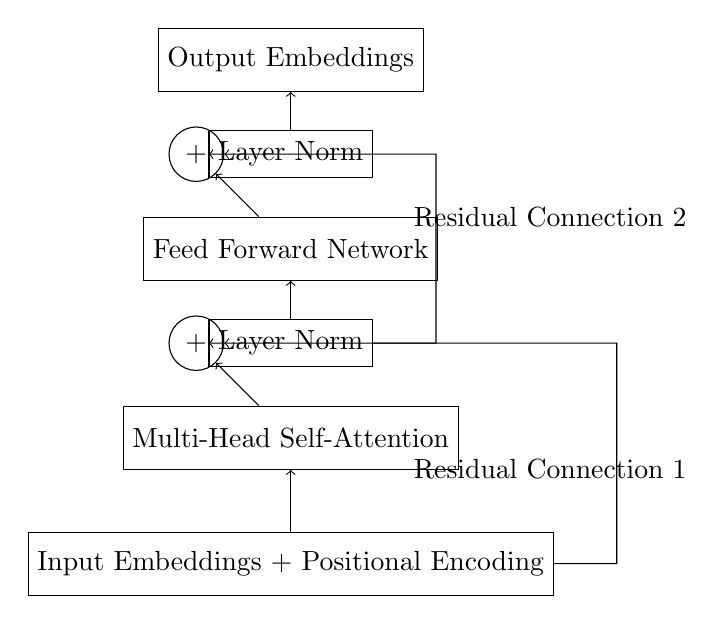
\begin{tikzpicture}[scale=0.8]
        % Input
        \node[rectangle, draw, minimum width=3cm, minimum height=0.8cm] (input) at (0, 0) {Input Embeddings + Positional Encoding};
        
        % Multi-head attention
        \node[rectangle, draw, minimum width=3cm, minimum height=0.8cm] (mha) at (0, 2) {Multi-Head Self-Attention};
        
        % Add & Norm 1
        \node[circle, draw, minimum size=0.6cm] (add1) at (-1.5, 3.5) {+};
        \node[rectangle, draw, minimum width=2cm, minimum height=0.6cm] (norm1) at (0, 3.5) {Layer Norm};
        
        % Feed Forward
        \node[rectangle, draw, minimum width=3cm, minimum height=0.8cm] (ff) at (0, 5) {Feed Forward Network};
        
        % Add & Norm 2
        \node[circle, draw, minimum size=0.6cm] (add2) at (-1.5, 6.5) {+};
        \node[rectangle, draw, minimum width=2cm, minimum height=0.6cm] (norm2) at (0, 6.5) {Layer Norm};
        
        % Output
        \node[rectangle, draw, minimum width=3cm, minimum height=0.8cm] (output) at (0, 8) {Output Embeddings};
        
        % Arrows
        \draw[->] (input) -- (mha);
        \draw[->] (mha) -- (add1);
        \draw[->] (add1) -- (norm1);
        \draw[->] (norm1) -- (ff);
        \draw[->] (ff) -- (add2);
        \draw[->] (add2) -- (norm2);
        \draw[->] (norm2) -- (output);
        
        % Skip connections
        \draw[->] (input.east) -- ++(1,0) -- ++(0,3.5) -- (add1.east);
        \draw[->] (norm1.east) -- ++(1,0) -- ++(0,3) -- (add2.east);
        
        % Labels
        \node[anchor=west] at (1.8, 1.5) {Residual Connection 1};
        \node[anchor=west] at (1.8, 5.5) {Residual Connection 2};
        
    \end{tikzpicture}
    \end{center}
    
    \answer{Complete transformer encoder block with multi-head attention, residual connections, and layer normalization.}
    
    \explanation{
    \textbf{Component Descriptions:}
    
    \textbf{1. Multi-Head Self-Attention:}
    \begin{itemize}
        \item Processes input embeddings with multiple attention heads
        \item Captures different types of relationships
        \item Output has same dimension as input
    \end{itemize}
    
    \textbf{2. Residual Connections (Skip Connections):}
    \begin{itemize}
        \item Direct path from input to addition point
        \item Helps gradient flow during backpropagation
        \item Enables training of deeper networks
        \item Formula: $\text{output} = \text{sublayer}(\text{input}) + \text{input}$
    \end{itemize}
    
    \textbf{3. Layer Normalization:}
    \begin{itemize}
        \item Normalizes features across embedding dimension
        \item Stabilizes training dynamics
        \item Applied after residual addition
        \item Formula: $\text{LayerNorm}(x) = \gamma \frac{x - \mu}{\sigma} + \beta$
    \end{itemize}
    
    \textbf{4. Feed-Forward Network:}
    \begin{itemize}
        \item Two linear transformations with ReLU activation
        \item Applied position-wise (same network for each position)
        \item Increases then decreases dimensionality
        \item $\text{FFN}(x) = \max(0, xW_1 + b_1)W_2 + b_2$
    \end{itemize}
    
    \textbf{Information Flow:}
    \begin{enumerate}
        \item Input embeddings + positional encoding
        \item Multi-head self-attention
        \item Add residual connection + layer normalization
        \item Feed-forward network
        \item Add residual connection + layer normalization
        \item Output embeddings (ready for next layer)
    \end{enumerate}
    }
    
    \item Explain the purpose of skip connections and layer normalization in the transformer architecture as discussed in the lecture. \hfill (5 marks)
    
    \answer{Skip connections enable gradient flow and layer normalization stabilizes training, together enabling deep transformer architectures.}
    
    \explanation{
    \textbf{Skip Connections (Residual Connections):}
    
    \textbf{Purpose:}
    \begin{itemize}
        \item Provide direct gradient flow path
        \item Enable identity mapping when needed
        \item Facilitate training of deep networks
        \item Prevent degradation problem
    \end{itemize}
    
    \textbf{How They Work:}
    \begin{itemize}
        \item $\text{output} = F(\text{input}) + \text{input}$
        \item Sublayer learns residual function $F$
        \item Easier to learn modifications than complete transformations
        \item Gradient flows directly through skip path
    \end{itemize}
    
    \textbf{Layer Normalization:}
    
    \textbf{Purpose:}
    \begin{itemize}
        \item Stabilize training dynamics
        \item Reduce internal covariate shift
        \item Enable higher learning rates
        \item Improve convergence speed
    \end{itemize}
    
    \textbf{How It Works:}
    \begin{itemize}
        \item Normalizes across feature dimension for each position
        \item Zero mean, unit variance for each embedding
        \item Learnable scale ($\gamma$) and shift ($\beta$) parameters
        \item Applied after residual addition
    \end{itemize}
    
    \textbf{Combined Benefits:}
    \begin{itemize}
        \item Enables training of 12+ layer transformers
        \item Stable gradients throughout the network
        \item Faster convergence and better final performance
        \item Robust to hyperparameter choices
    \end{itemize}
    }
\end{enumerate}

\vfill
\begin{center}{\bf END OF PAPER}\end{center>
\end{document}